\chapter{Histórias de Usuário} \label{cha:historiasUsuário}

Neste capítulo serão apresentadas as histórias de usuários definidas para o desenvolvimento deste software. As histórias são descritas de forma detalhada e contextualizada as necessidades, objetivos e requisitos específicos dos usuários em relação ao sistema. Cada história de usuário é uma narrativa curta que descreve uma funcionalidade. As histórias de usuário são uma ferramenta importante para o desenvolvimento ágil de software, pois permitem uma compreensão clara das expectativas dos usuários e fornecem direcionamento para o desenvolvimento incremental e iterativo do aplicativo.

\section{Buscar produto}%%%%%%%%%%%%%%%%%%%%%%%%%%%%%%%%%%%%%

\newcounter{numhistoria}
\setcounter{numhistoria}{1}
\newcommand{\nhist}{%
  \padzeroes[2]{\decimal{numhistoria}}%
  \stepcounter{numhistoria}%
}

%\begin{quadro}[hbt!]
%\centering
\begin{tabular}{|ll|}
\hline
\multicolumn{2}{|c|}{\textbf{UC\nhist - \currentname}}    \\ \hline
\multicolumn{1}{|l|}{\textbf{Sendo}}     & um usuário \\ \hline
\multicolumn{1}{|l|}{\textbf{Quero}}     & buscar um produto \\ \hline
\multicolumn{1}{|l|}{\textbf{Para}}      & encontrar oque tenha melhor preço e localização \\ \hline
\multicolumn{1}{|l|}{\textbf{Protótipo}} & 
\begin{minipage}{0.48\textwidth} 
\begin{figure}[H]
\caption{\label{fig:label} TELA INICIAL}
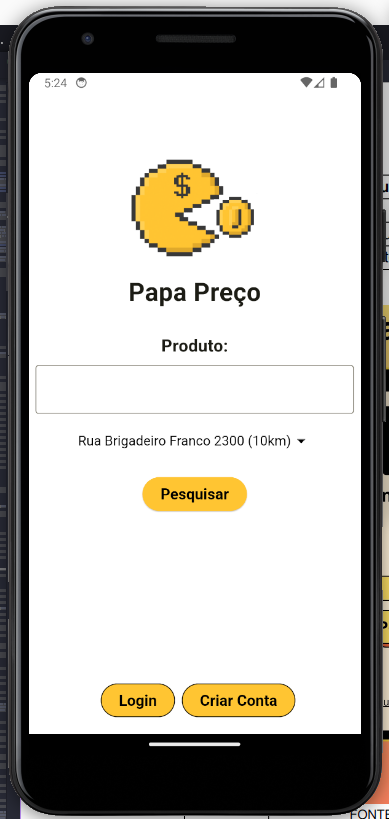
\includegraphics[width=.8\textwidth]{fig/telas/t_inicial.png}
\footnotesize \centering
\par FONTE: O Autor (2024)
\end{figure}
\end{minipage} \\ \hline
\end{tabular}
%\end{quadro}



\subsection*{\textbf{CRITÉRIOS DE ACEITAÇÃO}}

\begin{enumerate}[leftmargin=2cm]
    \item Deve permitir inserir o nome do produto.
    \item Deve definir a localização do usuário automaticamente por GPS.
    \item Deve permitir que o usuário troque a localização.
    \item Deve permitir que o usuário vá para a tela de login.
    \item Deve permitir que o usuário vá para a tela de criar conta.
    \item Deve buscar os produtos por nome.
\end{enumerate}

\subsection*{\textbf{CRITÉRIOS DE ACEITAÇÃO - DETALHAMENTO}}

\begin{tabularx}{0.9\textwidth}{|l|X|}
\multicolumn{2}{@{}l}{\textbf{1. Deve permitir inserir o nome do produto.}} \\ \hline
\textbf{Dado que} & Usuário está na tela de pesquisa. \\ \hline
\textbf{Quando} & Usuário clica no campo "Produto". \\ \hline
\textbf{Então} & Sistema permite a inserção do nome do produto. (R1)\\ \hline
\end{tabularx}

\begin{tabularx}{0.9\textwidth}{|l|X|}
\multicolumn{2}{@{}l}{\textbf{2. Deve definir a localização do usuário automaticamente por GPS.}} \\ \hline
\textbf{Dado que} & Usuário está na tela de pesquisa.\\ \hline
\textbf{Quando} & Usuário abre o aplicativo. \\ \hline
\textbf{Então} & Sistema obtém a localização do usuário através do GPS. \\ \hline
\end{tabularx}

\begin{tabularx}{0.9\textwidth}{|l|X|}
\multicolumn{2}{@{}l}{\textbf{3. Deve permitir que o usuário troque a localização.}} \\ \hline
\textbf{Dado que} & Usuário está na tela de pesquisa.\\ \hline
\textbf{Quando} & Usuário clica na localização atual. \\ \hline
\textbf{Então} & Sistema redireciona para a tela de definir nova localização. \\ \hline
\end{tabularx}

\begin{tabularx}{0.9\textwidth}{|l|X|}
\multicolumn{2}{@{}l}{\textbf{4. Deve permitir que o usuário vá para a tela de login.}} \\ \hline
\textbf{Dado que} & Usuário está na tela de pesquisa. \\ \hline
\textbf{Quando} & Usuário clica no botão "Login". \\ \hline
\textbf{Então} & Sistema redireciona para a tela de login. \\ \hline
\end{tabularx}

\begin{tabularx}{0.9\textwidth}{|l|X|}
\multicolumn{2}{@{}l}{\textbf{5. Deve permitir que o usuário vá para a tela de criar conta.}} \\ \hline
\textbf{Dado que} & Usuário está na tela de pesquisa. \\ \hline
\textbf{Quando} & Usuário lica no botão "Criar Conta". \\ \hline
\textbf{Então} & Sistema redireciona para a tela de cadastro. \\ \hline
\end{tabularx}

\begin{tabularx}{0.9\textwidth}{|l|X|}
\multicolumn{2}{@{}l}{\textbf{6. Deve buscar os produtos por nome.}} \\ \hline
\textbf{Dado que} & Usuário inseriu o nome de um produto. (R1) \\ \hline
\textbf{Quando} & Usuário clica em "Pesquisar". \\ \hline
\textbf{Então} & Sistema redireciona para a tela com os produtos buscados. \\ \hline
\end{tabularx}

\subsection*{\textbf{REGRAS DE NEGÓCIO DA HISTÓRIA}}

\begin{itemize}
    \item[] R1 - Tamanho máximo do texto 256 caracteres.
\end{itemize}

\section{Definir Localização}%%%%%%%%%%%%%%%%%%%%%%%%%%%%%%%%%%%%%

\begin{tabular}{|ll|}
\hline
\multicolumn{2}{|c|}{\textbf{UC\nhist - \currentname}}    \\ \hline
\multicolumn{1}{|l|}{\textbf{Sendo}}     & um usuário \\ \hline
\multicolumn{1}{|l|}{\textbf{Quero}}     & trocar a localização \\ \hline
\multicolumn{1}{|l|}{\textbf{Para}}      & especificar nas minhas buscas \\ \hline
\multicolumn{1}{|l|}{\textbf{Protótipo}} & 
\begin{minipage}{0.48\textwidth} 
\begin{figure}[H]
\caption{\label{fig:label} TELA DEFINIR LOCALIZACÃO}
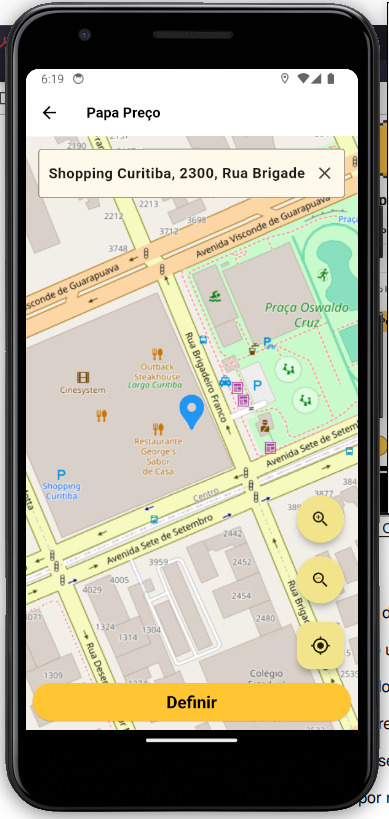
\includegraphics[width=.8\textwidth]{fig/telas/t_definirlocalizacao.png}
\footnotesize \centering
\par FONTE: O Autor (2024)
\end{figure}
\end{minipage} \\ \hline
\end{tabular}



\subsection*{\textbf{CRITÉRIOS DE ACEITAÇÃO}}

\begin{enumerate}[leftmargin=2cm]
    \item Deve permitir inserir o nome de uma localização.
    \item Deve permitir movimentar o marcador pelo mapa.
    \item Deve salvar a nova localização.
\end{enumerate}

\subsection*{\textbf{CRITÉRIOS DE ACEITAÇÃO - DETALHAMENTO}}

\begin{tabularx}{0.9\textwidth}{|l|X|}
\multicolumn{2}{@{}l}{\textbf{1. Deve permitir inserir o nome de uma localização.}} \\ \hline
\textbf{Dado que} & Usuário está na tela de definir localização. \\ \hline
\textbf{Quando} & Usuário clica no campo da localização atual. \\ \hline
\textbf{Então} & Sistema permite a inserção da nova localização. \\ \hline
\end{tabularx}

\begin{tabularx}{0.9\textwidth}{|l|X|}
\multicolumn{2}{@{}l}{\textbf{2. Deve permitir movimentar o marcador pelo mapa.}} \\ \hline
\textbf{Dado que} & Usuário está na tela de definir localização.\\ \hline
\textbf{Quando} & Usuário clica e arrasta no mapa. \\ \hline
\textbf{Então} & Sistema atualiza a localização com base na posição do marcador. \\ \hline
\end{tabularx}

\begin{tabularx}{0.9\textwidth}{|l|X|}
\multicolumn{2}{@{}l}{\textbf{3. Deve salvar a nova localização.}} \\ \hline
\textbf{Dado que} & Usuário está na tela de definir localização.\\ \hline
\textbf{Quando} & Usuário clica em "Definir". \\ \hline
\textbf{Então} & Sistema salva a nova localização. \\ \hline
\end{tabularx}

\section{Visualizar produtos}%%%%%%%%%%%%%%%%%%%%%%%%%%%%%%%%%%%%%

\begin{tabular}{|ll|}
\hline
\multicolumn{2}{|c|}{\textbf{UC\nhist - \currentname}}    \\ \hline
\multicolumn{1}{|l|}{\textbf{Sendo}}     & um usuário \\ \hline
\multicolumn{1}{|l|}{\textbf{Quero}}     & visualizar os produtos buscados\\ \hline
\multicolumn{1}{|l|}{\textbf{Para}}      & selecionar oque tenha melhor preço e localização \\ \hline
\multicolumn{1}{|l|}{\textbf{Protótipo}} & 
\begin{minipage}{0.48\textwidth} 
\begin{figure}[H]
\caption{\label{fig:label} TELA VISUALIZAR PRODUTOS}
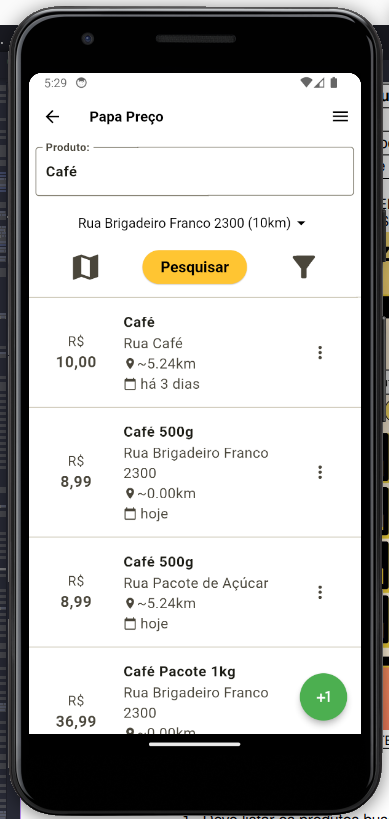
\includegraphics[width=.8\textwidth]{fig/telas/t_listarprod.png}
\footnotesize \centering
\par FONTE: O Autor (2024)
\end{figure}
\end{minipage}
 \\ \hline
\end{tabular}

\subsection*{\textbf{CRITÉRIOS DE ACEITAÇÃO}}

\begin{enumerate}[leftmargin=2cm]
    \item Deve listar os produtos buscados.
    \item Deve permitir fazer uma nova busca.
    \item Deve permitir que o usuário troque a localização.
    \item Deve permitir selecionar um produto na lista para mostrar mais detalhes.
    \item Deve permitir visualizar os produtos por mapa.
    \item Deve permitir filtrar a busca.
    \item Deve permitir adicionar novos produtos.
    \item Deve permitir usuário sugerir novo preço para um produto.
\end{enumerate}

\subsection*{\textbf{CRITÉRIOS DE ACEITAÇÃO - DETALHAMENTO}}
%\textbf{Critério de contexto} (Válido como premissa para todos os critérios):

%\begin{tabular}{@{}l l }
% \textbf{Dado que} & blabla \\ 
% \textbf{E} & blabla
%\end{tabular}

\begin{tabularx}{0.9\textwidth}{|l|X|}
\multicolumn{2}{@{}l}{\textbf{1. Deve listar os produtos buscados.}} \\ \hline
\textbf{Dado que} & Usuário pesquisou um produto valido. (R1)  \\ \hline
\textbf{Quando} & Sistema carrega a tela. \\ \hline
\textbf{Então} & Sistema apresenta a lista dos produtos encontrados.  \\ \hline
\end{tabularx}

\begin{tabularx}{0.9\textwidth}{|l|X|}
\multicolumn{2}{@{}l}{\textbf{2. Deve permitir fazer uma nova busca.}} \\ \hline
\textbf{Dado que} & Usuário inseriu o nome de um produto. (R2) \\ \hline
\textbf{Quando} & Usuário clica em "Pesquisar". \\ \hline
\textbf{Então} & Sistema carrega nova lista. \\ \hline
\end{tabularx}

\begin{tabularx}{0.9\textwidth}{|l|X|}
\multicolumn{2}{@{}l}{\textbf{3. Deve permitir que o usuário troque a localização.}} \\ \hline
\textbf{Dado que} & Usuário está na tela de pesquisa.\\ \hline
\textbf{Quando} & Usuário clica na localização atual. \\ \hline
\textbf{Então} & Sistema redireciona para a tela de definir nova localização. \\ \hline
\end{tabularx}

\begin{tabularx}{0.9\textwidth}{|l|X|}
\multicolumn{2}{@{}l}{\textbf{\makecell[l]{4. Deve permitir selecionar um produto na lista para mostrar mais \\detalhes.}}} \\
\hline \textbf{Dado que} & Sistema carregou ao menos 1 produto. (R1) \\ \hline
\textbf{Quando} & Usuário clica em um produto. \\ \hline
\textbf{Então} & Sistema redireciona para tela de detalhe. \\ \hline
\end{tabularx}

\begin{tabularx}{0.9\textwidth}{|l|X|}
\multicolumn{2}{@{}l}{\textbf{5. Deve permitir visualizar os produtos por mapa.}} \\ \hline
\textbf{Dado que} & Sistema carregou ao menos 1 produto. (R1) \\ \hline
\textbf{Quando} & Usuário clica no ícone de mapa de um produto. \\ \hline
\textbf{Então} & Sistema apresenta a visualização por mapa. \\ \hline
\end{tabularx}

\begin{tabularx}{0.9\textwidth}{|l|X|}
\multicolumn{2}{@{}l}{\textbf{6. Deve permitir filtrar a busca.}} \\ \hline
\textbf{Dado que} & Usuário está na tela de listagem. \\ \hline
\textbf{Quando} & Usuário clica no ícone de filtro. \\ \hline
\textbf{Então} & Sistema apresenta as opções de filtragem. \\ \hline
\end{tabularx}

\begin{tabularx}{0.9\textwidth}{|l|X|}
\multicolumn{2}{@{}l}{\textbf{7. Deve permitir adicionar novos produtos.}} \\ \hline
\textbf{Dado que} & Usuário está na tela de listagem. \\ \hline
\textbf{Quando} & Usuário clica no ícone de adicionar. (R3) \\ \hline
\textbf{Então} & Sistema redireciona para tela de cadastro de produto. \\ \hline
\end{tabularx}

\begin{tabularx}{0.9\textwidth}{|l|X|}
\multicolumn{2}{@{}l}{\textbf{8. Deve permitir usuário sugerir novo preço para um produto.}} \\ \hline
\textbf{Dado que} & Usuário está na tela de listagem. \\ \hline
\textbf{Quando} & Usuário clica na opção de sugerir novo preço de um determinado produto. (R3) \\ \hline
\textbf{Então} & Sistema redireciona para tela de sugerir novo preço. \\ \hline
\end{tabularx}

\subsection*{\textbf{REGRAS DE NEGÓCIO DA HISTÓRIA}}

\begin{itemize}
    \item[] R1 - Produto cadastrado no banco de dados.
    \item[] R2 - Tamanho máximo do texto 256 caracteres.
    \item[] R3 - Usuário precisa estar logado.
\end{itemize}

\section{Visualizar mapa}%%%%%%%%%%%%%%%%%%%%%%%%%%%%%%%%%%%%%

\begin{tabular}{|ll|}
\hline
\multicolumn{2}{|c|}{\textbf{UC\nhist - \currentname}}    \\ \hline
\multicolumn{1}{|l|}{\textbf{Sendo}}     & um usuário \\ \hline
\multicolumn{1}{|l|}{\textbf{Quero}}     & visualizar os produtos buscados no mapa\\ \hline
\multicolumn{1}{|l|}{\textbf{Para}}      & verificar no mapa a localização dos produtos\\ \hline
\multicolumn{1}{|l|}{\textbf{Protótipo}} & 
\begin{minipage}{0.48\textwidth} 
\begin{figure}[H]
\caption{\label{fig:label} TELA MAPA}
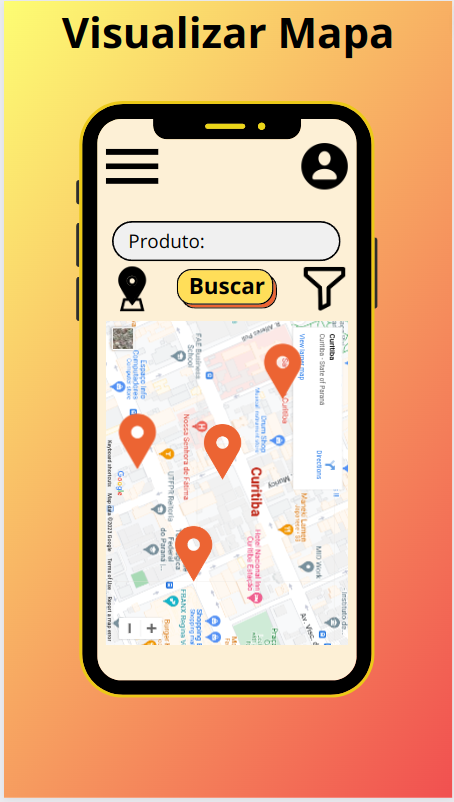
\includegraphics[width=.8\textwidth]{fig/telas/t_mapa.png}
\footnotesize \centering
\par FONTE: O Autor (2024)
\end{figure}
\end{minipage}
 \\ \hline
\end{tabular}

\subsection*{\textbf{CRITÉRIOS DE ACEITAÇÃO}}

\begin{enumerate}[leftmargin=2cm]
    \item Deve mostrar os produtos buscados em suas respectivas localizações no mapa. (R1)
    \item Deve permitir selecionar um produto no mapa para mostrar mais detalhes.
\end{enumerate}

\subsection*{\textbf{CRITÉRIOS DE ACEITAÇÃO - DETALHAMENTO}}


\begin{tabularx}{0.9\textwidth}{|l|X|}
\multicolumn{2}{@{}l}{\textbf{\makecell[l]{1. Deve mostrar os produtos buscados em suas respectivas \\localizações no mapa.}}} \\ \hline
\textbf{Dado que} & Usuário buscou produtos. \\ \hline
\textbf{Quando} & Usuário está na tela do mapa. \\ \hline
\textbf{Então} & Sistema mostra os produtos em seus respectivos locais no mapa. \\ \hline
\end{tabularx}

\begin{tabularx}{0.9\textwidth}{|l|X|}
\multicolumn{2}{@{}l}{\textbf{\makecell[l]{2. Deve permitir selecionar um produto no mapa para mostrar mais \\detalhes.}}} \\ \hline
\textbf{Dado que} & Sistema encontrou 1 produto. (R1) \\ \hline
\textbf{Quando} & Usuário seleciona um produto no mapa. \\ \hline
\textbf{Então} & Sistema redireciona para tela de detalhe. \\ \hline
\end{tabularx}

\subsection*{\textbf{REGRAS DE NEGÓCIO DA HISTÓRIA}}

\begin{itemize}
    \item[] R1 - Produto cadastrado no banco de dados.
\end{itemize}


\section{Filtrar busca produtos}%%%%%%%%%%%%%%%%%%%%%%%%%%%%%%%%%%%%%

\begin{tabular}{|ll|}
\hline
\multicolumn{2}{|c|}{\textbf{UC\nhist - \currentname}}    \\ \hline
\multicolumn{1}{|l|}{\textbf{Sendo}}     & um usuário \\ \hline
\multicolumn{1}{|l|}{\textbf{Quero}}     & filtrar a minha busca\\ \hline
\multicolumn{1}{|l|}{\textbf{Para}}      & encontrar um produto especificando os parâmetros da busca\\ \hline
\multicolumn{1}{|l|}{\textbf{Protótipo}} & 
\begin{minipage}{0.48\textwidth} 
\begin{figure}[H]
\caption{\label{fig:label} TELA FILTRAR BUSCA}
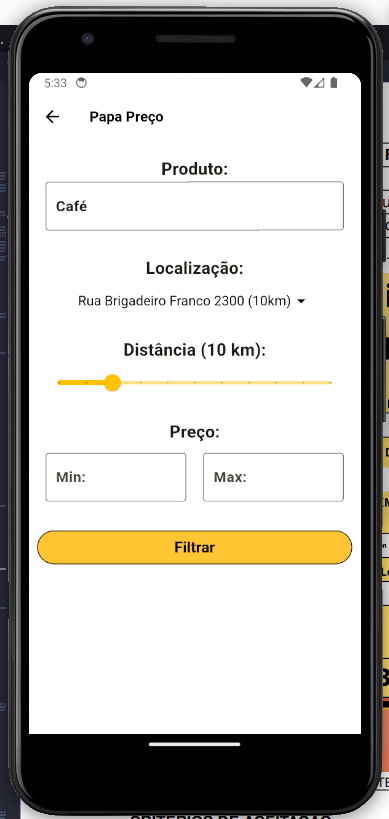
\includegraphics[width=.8\textwidth]{fig/telas/t_filtros.png}
\footnotesize \centering
\par FONTE: O Autor (2024)
\end{figure}
\end{minipage}
 \\ \hline
\end{tabular}

\subsection*{\textbf{CRITÉRIOS DE ACEITAÇÃO}}

\begin{enumerate}[leftmargin=2cm]
    \item Deve permitir inserir o nome do produto.
    \item Deve permitir especificar a distância máxima.
    \item Deve permitir especificar o preço mínimo e máximo.
    \item Deve permitir especificar a localização do produto.
\end{enumerate}

\subsection*{\textbf{CRITÉRIOS DE ACEITAÇÃO - DETALHAMENTO}}


\begin{tabularx}{0.9\textwidth}{|l|X|}
\multicolumn{2}{@{}l}{\textbf{1. Deve permitir inserir o nome do produto.}} \\ \hline
\textbf{Dado que} & Usuário clicou no ícone de filtro. \\ \hline
\textbf{Quando} & Usuário clica no campo "Produto". \\ \hline
\textbf{Então} & Sistema permite inserir nome de um produto. (R1)\\ \hline
\end{tabularx}

\begin{tabularx}{0.9\textwidth}{|l|X|}
\multicolumn{2}{@{}l}{\textbf{2. Deve permitir especificar a distância máxima.}} \\ \hline
\textbf{Dado que} & Usuário clicou no ícone de filtro. \\ \hline
\textbf{Quando} & Usuário clica no campo "Distância". \\ \hline
\textbf{Então} & Sistema permite inserir distância. (R2) \\ \hline
\end{tabularx}

\begin{tabularx}{0.9\textwidth}{|l|X|}
\multicolumn{2}{@{}l}{\textbf{3. Deve permitir especificar o preço mínimo e máximo.}} \\ \hline
\textbf{Dado que} & Usuário clicou no ícone de filtro. \\ \hline
\textbf{Quando} & Usuário clica no campo "Preço". \\ \hline
\textbf{Então} & Sistema permite inserir preço mínimo e máximo. (R3) \\ \hline
\end{tabularx}

\begin{tabularx}{0.9\textwidth}{|l|X|}
\multicolumn{2}{@{}l}{\textbf{4. Deve permitir especificar a localização do produto.}} \\ \hline
\textbf{Dado que} & Usuário clicou no ícone de filtro  \\ \hline
\textbf{Quando} & Usuário clica no campo "Localização". \\ \hline
\textbf{Então} & Sistema permite inserir localização. (R4) \\ \hline
\end{tabularx}

\subsection*{\textbf{REGRAS DE NEGÓCIO DA HISTÓRIA}}

\begin{itemize}
    \item[] R1 - Tamanho máximo do texto 256 caracteres.
    \item[] R2 - Distância mínima 5km, distância máxima 50km.
    \item[] R3 - Preço mínimo 0, preço máximo 999,999.
    \item[] R4 - CEP válido ou localização no mapa.
\end{itemize}



\section{Detalhes produto}%%%%%%%%%%%%%%%%%%%%%%%%%%%%%%%%%%%%%

\begin{tabular}{|ll|}
\hline
\multicolumn{2}{|c|}{\textbf{UC\nhist - \currentname}}    \\ \hline
\multicolumn{1}{|l|}{\textbf{Sendo}}     & um usuário \\ \hline
\multicolumn{1}{|l|}{\textbf{Quero}}     & visualizar os detalhes do produto\\ \hline
\multicolumn{1}{|l|}{\textbf{Para}}      & analisar a localização e preço do produto\\ \hline
\multicolumn{1}{|l|}{\textbf{Protótipo}} & 
\begin{minipage}{0.48\textwidth} 
\begin{figure}[H]
\caption{\label{fig:label} TELA DETALHES PRODUTO}
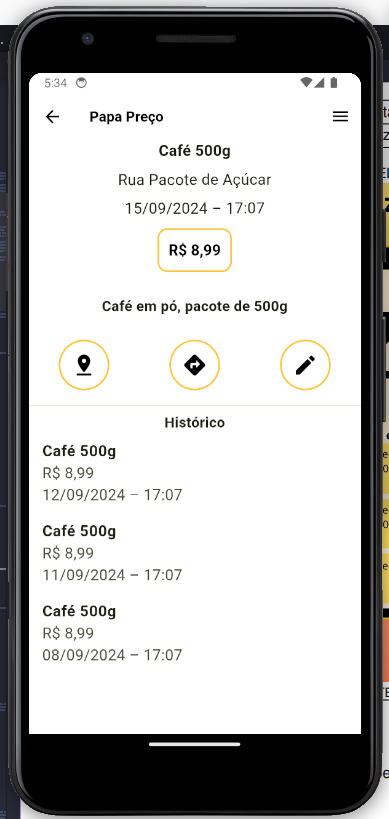
\includegraphics[width=.8\textwidth]{fig/telas/t_produto.png}
\footnotesize \centering
\par FONTE: O Autor (2024)
\end{figure}
\end{minipage}
 \\ \hline
\end{tabular}

\subsection*{\textbf{CRITÉRIOS DE ACEITAÇÃO}}

\begin{enumerate}[leftmargin=2cm]
    \item Deve mostrar as informações do produto como: nome, preço, localização e data da observação.
    \item Deve mostrar histórico de preços do produto.
    \item Deve permitir mostrar o localização no mapa.
    \item Deve permitir traçar rota no Google Maps.
    \item Deve permitir sugerir um novo preço para o produto no estabelecimento.
\end{enumerate}

\subsection*{\textbf{CRITÉRIOS DE ACEITAÇÃO - DETALHAMENTO}}
\textbf{Critério de contexto} (Válido como premissa para todos os critérios):

\begin{tabularx}{0.9\textwidth}{@{}l X }
 \textbf{Dado que} & Sistema buscou ao menos 1 produto. \\ 
 \textbf{E} & Usuário clicou em 1 produto.
\end{tabularx}


\begin{tabularx}{0.9\textwidth}{|l|X|}
\multicolumn{2}{@{}l}{\textbf{\makecell[l]{1. Deve mostrar as informações do produto como: nome, \\preço, localização e data da observação.}}} \\ \hline
\textbf{Dado que} & Usuário está na tela de detalhe. \\ \hline
\textbf{Quando} & Sistema carrega informações do produto. \\ \hline
\textbf{Então} & Sistema apresenta informações do produto. \\ \hline
\end{tabularx}

\begin{tabularx}{0.9\textwidth}{|l|X|}
\multicolumn{2}{@{}l}{\textbf{\makecell[l]{2. Deve mostrar histórico de preços do produto.}}} \\ \hline
\textbf{Dado que} & Usuário está na tela de detalhe. \\ \hline
\textbf{Quando} & Sistema carrega informações do produto. \\ \hline
\textbf{Então} & Sistema apresenta histórico de preço do produto. \\ \hline
\end{tabularx}

\begin{tabularx}{0.9\textwidth}{|l|X|}
\multicolumn{2}{@{}l}{\textbf{3. Deve permitir mostrar o localização no mapa.}} \\ \hline
\textbf{Dado que} & Usuário está na tela de detalhe. \\ \hline
\textbf{Quando} & Usuário clica no ícone do mapa. \\ \hline
\textbf{Então} & Sistema apresenta a localização do produto no mapa. \\ \hline
\end{tabularx}

\begin{tabularx}{0.9\textwidth}{|l|X|}
\multicolumn{2}{@{}l}{\textbf{4. Deve permitir traçar rota no Google Maps.}} \\ \hline
\textbf{Dado que} & Usuário está na tela de detalhe. \\ \hline
\textbf{Quando} & Usuário clica no ícone de navegação. \\ \hline
\textbf{Então} & Sistema redireciona para o Google Maps. \\ \hline
\end{tabularx}

\begin{tabularx}{0.9\textwidth}{|l|X|}
\multicolumn{2}{@{}l}{\textbf{\makecell[l]{5. Deve permitir sugerir um novo preço para o produto no \\estabelecimento.}}} \\ \hline
\textbf{Dado que} & Usuário está na tela de detalhe. \\ \hline
\textbf{Quando} & Usuário clica no botão de sugestão. (R1) \\ \hline
\textbf{Então} & Sistema apresenta formulário de sugestão de preço. \\ \hline
\end{tabularx}

\subsection*{\textbf{REGRAS DE NEGÓCIO DA HISTÓRIA}}

\begin{itemize}
    \item[] R1 - Usuário deve estar logado.
\end{itemize}


\section{Sugerir edição}%%%%%%%%%%%%%%%%%%%%%%%%%%%%%%%%%%%%%

\begin{tabular}{|ll|}
\hline
\multicolumn{2}{|c|}{\textbf{UC\nhist - \currentname}}    \\ \hline
\multicolumn{1}{|l|}{\textbf{Sendo}}     & um usuário \\ \hline
\multicolumn{1}{|l|}{\textbf{Quero}}     & sugerir a edição de preço de um produto\\ \hline
\multicolumn{1}{|l|}{\textbf{Para}}      & para que o produto apareça com o novo preço atualizado\\ \hline
\multicolumn{1}{|l|}{\textbf{Protótipo}} & 
\begin{minipage}{0.48\textwidth} 
\begin{figure}[H]
\caption{\label{fig:label} TELA SUGERIR EDIÇÃO}
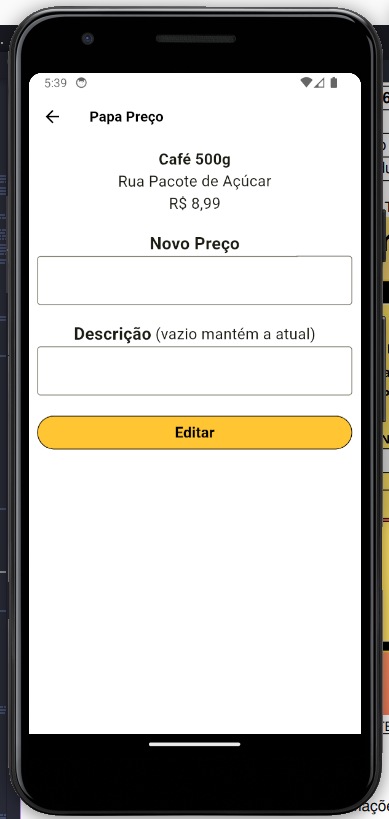
\includegraphics[width=.8\textwidth]{fig/telas/t_sugerir.png}
\footnotesize \centering
\par FONTE: O Autor (2024)
\end{figure}
\end{minipage}
 \\ \hline
\end{tabular}

\subsection*{\textbf{CRITÉRIOS DE ACEITAÇÃO}}

\begin{enumerate}[leftmargin=2cm]
    \item Deve mostrar as informações do produto.
    \item Deve permitir inserir um novo preço e descrição.
    \item Deve permitir sugerir um novo preço.
\end{enumerate}

\subsection*{\textbf{CRITÉRIOS DE ACEITAÇÃO - DETALHAMENTO}}
\textbf{Critério de contexto} (Válido como premissa para todos os critérios):

\begin{tabularx}{0.9\textwidth}{@{}l X }
\textbf{Dado que} & Sistema buscou ao menos 1 produto.\\ 
\textbf{E} & Usuário clicou em 1 produto.\\
\textbf{E} & Usuário clicou no botão de sugestão.
\end{tabularx}


\begin{tabularx}{0.9\textwidth}{|l|X|}
\multicolumn{2}{@{}l}{\textbf{1. Deve mostrar as informações do produto.}} \\ \hline
\textbf{Dado que} & Usuário está na tela de sugestão. \\ \hline
\textbf{Quando} & Sistema carrega informações do produto. \\ \hline
\textbf{Então} & Sistema apresenta informações atuais do produto. \\ \hline
\end{tabularx}

\begin{tabularx}{0.9\textwidth}{|l|X|}
\multicolumn{2}{@{}l}{\textbf{2. Deve permitir inserir um novo preço e descrição.}} \\ \hline
\textbf{Dado que} & Usuário está na tela de sugestão. \\ \hline
\textbf{Quando} & Usuário clica no campo "Novo preço" e "Descrição. \\ \hline
\textbf{Então} & Sistema permite inserir novo preço e descrição. (R1) \\ \hline
\end{tabularx}

\begin{tabularx}{0.9\textwidth}{|l|X|}
\multicolumn{2}{@{}l}{\textbf{3. Deve permitir sugerir um novo preço.}} \\ \hline
\textbf{Dado que} & Usuário inseriu preço válido. (R1) \\ \hline
\textbf{Quando} & Usuário clica no botão "Editar". \\ \hline
\textbf{Então} & Sistema cadastra nova sugestão. \\ \hline
\end{tabularx}

\subsection*{\textbf{REGRAS DE NEGÓCIO DA HISTÓRIA}}

\begin{itemize}
    \item[] R1 - Preço mínimo 0, preço máximo 999,999.
\end{itemize}


\section{Avaliar sugestão}%%%%%%%%%%%%%%%%%%%%%%%%%%%%%%%%%%%%%

\begin{tabular}{|ll|}
\hline
\multicolumn{2}{|c|}{\textbf{UC\nhist - \currentname}}    \\ \hline
\multicolumn{1}{|l|}{\textbf{Sendo}}     & um usuário \\ \hline
\multicolumn{1}{|l|}{\textbf{Quero}}     & avaliar uma sugestão de novo preço\\ \hline
\multicolumn{1}{|l|}{\textbf{Para}}      & para que o produto fique com o preço atualizado\\ \hline
\multicolumn{1}{|l|}{\textbf{Protótipo}} & 
\begin{minipage}{0.48\textwidth} 
\begin{figure}[H]
\caption{\label{fig:label} TELA AVALIAR SUGESTÃO}
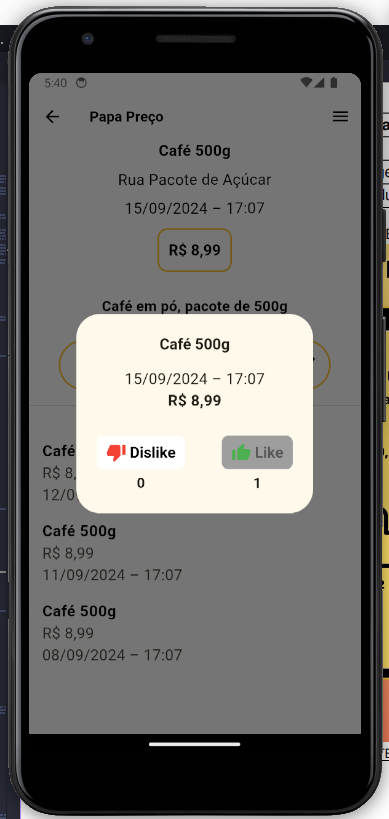
\includegraphics[width=.8\textwidth]{fig/telas/t_avaliar.png}
\footnotesize \centering
\par FONTE: O Autor (2024)
\end{figure}
\end{minipage}
 \\ \hline
\end{tabular}

\subsection*{\textbf{CRITÉRIOS DE ACEITAÇÃO}}

\begin{enumerate}[leftmargin=2cm]
    \item Deve mostrar as informações do produto.
    \item Deve permitir avaliar a sugestão com um positivo ou negativo.
    \item Deve atualizar o preço do produto se maioria das avaliações forem positivas.
\end{enumerate}

\subsection*{\textbf{CRITÉRIOS DE ACEITAÇÃO - DETALHAMENTO}}
\textbf{Critério de contexto} (Válido como premissa para todos os critérios):

\begin{tabularx}{0.9\textwidth}{@{}l X }
\textbf{Dado que} & Sistema buscou ao menos 1 produto. \\ 
\textbf{E} & Usuário clicou em 1 produto.
\end{tabularx}


\begin{tabularx}{0.9\textwidth}{|l|X|}
\multicolumn{2}{@{}l}{\textbf{\makecell[l]{1. Deve mostrar as informações do produto.}}} \\ \hline
\textbf{Dado que} & Usuário está na tela de avaliação. \\ \hline
\textbf{Quando} & Sistema carrega informações do produto. \\ \hline
\textbf{Então} & Sistema apresenta informações da sugestão. \\ \hline
\end{tabularx}

\begin{tabularx}{0.9\textwidth}{|l|X|}
\multicolumn{2}{@{}l}{\textbf{2. Deve permitir avaliar a sugestão com um positivo ou negativo.}} \\ \hline
\textbf{Dado que} & Usuário está na tela de avaliação. \\ \hline
\textbf{Quando} & Usuário avalia uma sugestão. \\ \hline
\textbf{Então} & Sistema atualiza números de avaliações. \\ \hline
\end{tabularx}

\begin{tabularx}{0.9\textwidth}{|l|X|}
\multicolumn{2}{@{}l}{\textbf{\makecell[l]{3. Deve atualizar o preço do produto se maioria das avaliações forem \\positivas.}}} \\ \hline
\textbf{Dado que} & Usuário está na tela de avaliação.  \\ \hline
\textbf{Quando} & Usuário avalia uma sugestão. \\ \hline
\textbf{Então} & Sistema atualiza preço do produto. (R1) \\ \hline
\end{tabularx}

\subsection*{\textbf{REGRAS DE NEGÓCIO DA HISTÓRIA}}

\begin{itemize}
    \item[] R1 - Diferença entre avaliações positiva.
\end{itemize}


\section{Cadastrar produto}%%%%%%%%%%%%%%%%%%%%%%%%%%%%%%%%%%%%%

\begin{tabular}{|ll|}
\hline
\multicolumn{2}{|c|}{\textbf{UC\nhist - \currentname}}    \\ \hline
\multicolumn{1}{|l|}{\textbf{Sendo}}     & um usuário \\ \hline
\multicolumn{1}{|l|}{\textbf{Quero}}     & cadastrar um novo produto\\ \hline
\multicolumn{1}{|l|}{\textbf{Para}}      & para que o produto apareça no sistema\\ \hline
\multicolumn{1}{|l|}{\textbf{Protótipo}} & 
\begin{minipage}{0.48\textwidth} 
\begin{figure}[H]
\caption{\label{fig:label} TELA CADASTRAR PRODUTO}
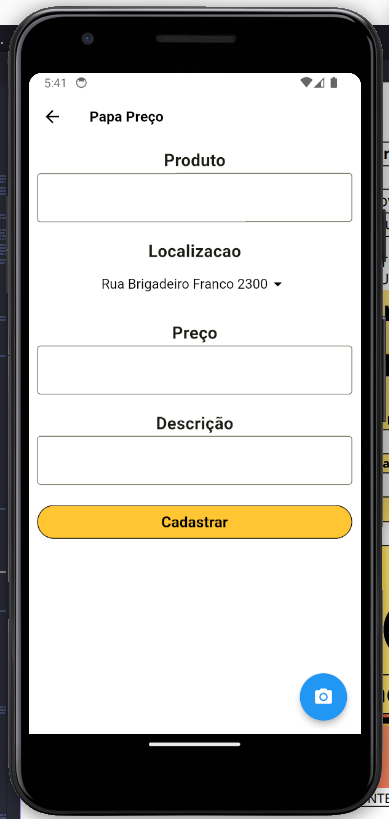
\includegraphics[width=.8\textwidth]{fig/telas/t_novproduto.png}
\footnotesize \centering
\par FONTE: O Autor (2024)
\end{figure}
\end{minipage}
 \\ \hline
\end{tabular}

\subsection*{\textbf{CRITÉRIOS DE ACEITAÇÃO}}

\begin{enumerate}[leftmargin=2cm]
    \item Deve permitir inserir o nome do produto, localização e preço do produto.
    \item Deve cadastrar o produto.
    \item Deve criar uma sugestão de novo preço pro produto caso já esteja cadastrado.
\end{enumerate}

\subsection*{\textbf{CRITÉRIOS DE ACEITAÇÃO - DETALHAMENTO}}
\textbf{Critério de contexto} (Válido como premissa para todos os critérios):

\begin{tabularx}{0.9\textwidth}{@{}l X }
 \textbf{Dado que} & Usuário esta logado \\ 
 \textbf{E} & Clicou no botão "Cadastrar produto".
\end{tabularx}

\begin{tabularx}{0.9\textwidth}{|l|X|}
\multicolumn{2}{@{}l}{\textbf{\makecell[l]{1. Deve permitir inserir o nome do produto, localização e \\preço do produto.}}} \\ \hline
\textbf{Dado que} & Usuário na tela de cadastro. \\ \hline
\textbf{Quando} & Usuário clica em algum campo. \\ \hline
\textbf{Então} & Sistema permite edição. \\ \hline
\end{tabularx}

\begin{tabularx}{0.9\textwidth}{|l|X|}
\multicolumn{2}{@{}l}{\textbf{2. Deve cadastrar o produto.}} \\ \hline
\textbf{Dado que} & Usuário inseriu dados corretamente. (R1) (R2) \\ \hline
\textbf{Quando} & Usuário clica no botão "Cadastrar". \\ \hline
\textbf{Então} & Sistema cadastra produto. \\ \hline
\end{tabularx}

\begin{tabularx}{0.9\textwidth}{|l|X|}
\multicolumn{2}{@{}l}{\textbf{\makecell[l]{3. Deve criar uma sugestão de novo preço pro produto caso já esteja \\cadastrado.}}} \\ \hline
\textbf{Dado que} & Usuário inseriu dados corretamente. (R1) (R2) \\ \hline
\textbf{Quando} & Produto já cadastrado na localização. \\ \hline
\textbf{Então} & Sistema cadastra sugestão de preço. \\ \hline
\end{tabularx}

\subsection*{\textbf{REGRAS DE NEGÓCIO DA HISTÓRIA}}

\begin{itemize}
    \item[] R1 - Localização correta no mapa.
    \item[] R2 - Preço mínimo 0, preço máximo 999,999.
\end{itemize}


\section{Digitalizar nota}%%%%%%%%%%%%%%%%%%%%%%%%%%%%%%%%%%%%%

\begin{tabular}{|ll|}
\hline
\multicolumn{2}{|c|}{\textbf{UC\nhist - \currentname}}    \\ \hline
\multicolumn{1}{|l|}{\textbf{Sendo}}     & um usuário \\ \hline
\multicolumn{1}{|l|}{\textbf{Quero}}     & digitalizar uma nota\\ \hline
\multicolumn{1}{|l|}{\textbf{Para}}      & para inserir automaticamente os produtos no sistema\\ \hline
\multicolumn{1}{|l|}{\textbf{Protótipo}} & 
\begin{minipage}{0.48\textwidth} 
\begin{figure}[H]
\caption{\label{fig:label} TELA DIGITALIZAR}
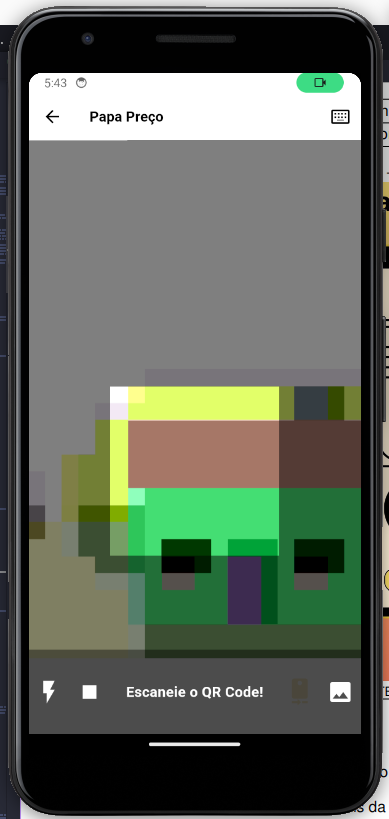
\includegraphics[width=.8\textwidth]{fig/telas/t_digitaliza.png}
\footnotesize \centering
\par FONTE: O Autor (2024)
\end{figure}
\end{minipage}
 \\ \hline
\end{tabular}

\subsection*{\textbf{CRITÉRIOS DE ACEITAÇÃO}}

\begin{enumerate}[leftmargin=2cm]
    \item Deve permitir tirar uma foto de uma nota fiscal.
    \item Deve permitir escolher uma foto da galeria.
    \item Deve permitir digitar a URL do QRCode.
    \item Deve digitalizar os itens da nota em texto.
    \item Deve permitir ligar o flash do celular.
\end{enumerate}

\subsection*{\textbf{CRITÉRIOS DE ACEITAÇÃO - DETALHAMENTO}}
\textbf{Critério de contexto} (Válido como premissa para todos os critérios):

\begin{tabularx}{0.9\textwidth}{@{}l X }
\textbf{Dado que} & Usuário esta logado \\ 
\textbf{E} & Clicou no botão "Cadastrar produto".\\
\textbf{E} & Clicou no ícone de nota fiscal.
\end{tabularx}


\begin{tabularx}{0.9\textwidth}{|l|X|}
\multicolumn{2}{@{}l}{\textbf{1. Deve permitir tirar uma foto de uma nota fiscal.}} \\ \hline
\textbf{Dado que} & Usuário está na tela de nota fiscal. \\ \hline
\textbf{Quando} & Usuário clica no ícone de camera. \\ \hline
\textbf{Então} & Sistema permite escanear uma foto. \\ \hline
\end{tabularx}

\begin{tabularx}{0.9\textwidth}{|l|X|}
\multicolumn{2}{@{}l}{\textbf{2. Deve permitir escolher uma foto da galeria.}} \\ \hline
\textbf{Dado que} & Usuário está na tela de nota fiscal. \\ \hline
\textbf{Quando} & Usuário clica no ícone de foto. \\ \hline
\textbf{Então} & Sistema permite selecionar uma foto da galeria. \\ \hline
\end{tabularx}

\begin{tabularx}{0.9\textwidth}{|l|X|}
\multicolumn{2}{@{}l}{\textbf{3. Deve permitir digitar a URL do QRCode.}} \\ \hline
\textbf{Dado que} & Usuário está na tela de nota fiscal. \\ \hline
\textbf{Quando} & Usuário clica no ícone de teclado. \\ \hline
\textbf{Então} & Sistema permite digitar a URL. \\ \hline
\end{tabularx}

\begin{tabularx}{0.9\textwidth}{|l|X|}
\multicolumn{2}{@{}l}{\textbf{4. Deve digitalizar os itens da nota em texto.}} \\ \hline
\textbf{Dado que} & Usuário escaneou nota corretamente. (R1) \\ \hline
\textbf{Quando} & Usuário clica no ícone de camera. \\ \hline
\textbf{Então} & Sistema redireciona para tela de confirmação. \\ \hline
\end{tabularx}

\begin{tabularx}{0.9\textwidth}{|l|X|}
\multicolumn{2}{@{}l}{\textbf{5. Deve permitir ligar o flash do celular.}} \\ \hline
\textbf{Dado que} & Usuário está na tela de nota fiscal. \\ \hline
\textbf{Quando} & Usuário clica no ícone de flash. \\ \hline
\textbf{Então} & Sistema liga o flash do celular. \\ \hline
\end{tabularx}

\subsection*{\textbf{REGRAS DE NEGÓCIO DA HISTÓRIA}}

\begin{itemize}
    \item[] R1 - QR Code da nota fiscal encontrada.
\end{itemize}

\section{Confirmar digitalização}%%%%%%%%%%%%%%%%%%%%%%%%%%%%%%%%%%%%%

\begin{tabular}{|ll|}
\hline
\multicolumn{2}{|c|}{\textbf{UC\nhist - \currentname}}    \\ \hline
\multicolumn{1}{|l|}{\textbf{Sendo}}     & um usuário \\ \hline
\multicolumn{1}{|l|}{\textbf{Quero}}     & confirmar a digitalização\\ \hline
\multicolumn{1}{|l|}{\textbf{Para}}      & para corrigir eventuais erros inseridos pelo sistema\\ \hline
\multicolumn{1}{|l|}{\textbf{Protótipo}} & 
\begin{minipage}{0.48\textwidth} 
\begin{figure}[H]
\caption{\label{fig:label} TELA DIGITALIZAÇÃO}
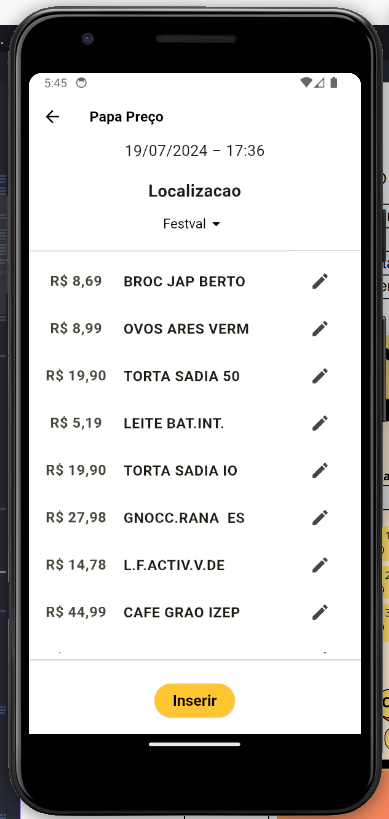
\includegraphics[width=.8\textwidth]{fig/telas/t_confdigitaliza.png}
\footnotesize \centering
\par FONTE: O Autor (2024)
\end{figure}
\end{minipage}
 \\ \hline
\end{tabular}

\subsection*{\textbf{CRITÉRIOS DE ACEITAÇÃO}}

\begin{enumerate}[leftmargin=2cm]
    \item Deve permitir inserir a localização da nota.
    \item Deve permitir alterar os produtos digitalizados pelo sistema.
    \item Deve cadastrar os produtos.
    \item Deve criar uma sugestão de novo preço pro produto caso já esteja cadastrado.
\end{enumerate}

\subsection*{\textbf{CRITÉRIOS DE ACEITAÇÃO - DETALHAMENTO}}
\textbf{Critério de contexto} (Válido como premissa para todos os critérios):

\begin{tabularx}{0.9\textwidth}{@{}l X }
\textbf{Dado que} & Usuário esta logado \\ 
\textbf{E} & Clicou no botão "Cadastrar produto".\\
\textbf{E} & Clicou no ícone de nota fiscal.\\
\textbf{E} & Escaneou uma nota válida.
\end{tabularx}


\begin{tabularx}{0.9\textwidth}{|l|X|}
\multicolumn{2}{@{}l}{\textbf{1. Deve permitir inserir a localização da nota.}} \\ \hline
\textbf{Dado que} & Usuário está na tela de confirmação. \\ \hline
\textbf{Quando} & Usuário clica no campo "Localização". \\ \hline
\textbf{Então} & Sistema permite selecionar no mapa a localiação. \\ \hline
\end{tabularx}

\begin{tabularx}{0.9\textwidth}{|l|X|}
\multicolumn{2}{@{}l}{\textbf{2. Deve permitir alterar os produtos digitalizados pelo sistema.}} \\ \hline
\textbf{Dado que} & Usuário está na tela de confirmação. \\ \hline
\textbf{Quando} & Usuário clica no ícone de edição. \\ \hline
\textbf{Então} & Sistema apresenta formulário de edição. \\ \hline
\end{tabularx}

\begin{tabularx}{0.9\textwidth}{|l|X|}
\multicolumn{2}{@{}l}{\textbf{3. Deve cadastrar os produtos.}} \\ \hline
\textbf{Dado que} & Usuário está na tela de confirmação. \\ \hline
\textbf{Quando} & Usuário clica no ícone "Confirmar". \\ \hline
\textbf{Então} & Sistema cadastra produtos. \\ \hline
\end{tabularx}

\begin{tabularx}{0.9\textwidth}{|l|X|}
\multicolumn{2}{@{}l}{\textbf{\makecell[l]{4. Deve criar uma sugestão de novo preço pro produto caso já esteja \\cadastrado.}}} \\ \hline
\textbf{Dado que} & Usuário clica no ícone "Confirmar".\\ \hline
\textbf{Quando} & Produto já cadastrado. \\ \hline
\textbf{Então} & Sistema cadastra sugestão de novo preço. \\ \hline
\end{tabularx}


\section{Menu perfil}%%%%%%%%%%%%%%%%%%%%%%%%%%%%%%%%%%%%%

\begin{tabular}{|ll|}
\hline
\multicolumn{2}{|c|}{\textbf{UC\nhist - \currentname}}    \\ \hline
\multicolumn{1}{|l|}{\textbf{Sendo}}     & um usuário \\ \hline
\multicolumn{1}{|l|}{\textbf{Quero}}     & visualizar os detalhes do meu perfil\\ \hline
\multicolumn{1}{|l|}{\textbf{Para}}      & alterar minha senha ou foto\\ \hline
\multicolumn{1}{|l|}{\textbf{Protótipo}} & 
\begin{minipage}{0.48\textwidth} 
\begin{figure}[H]
\caption{\label{fig:label} TELA PERFIL}
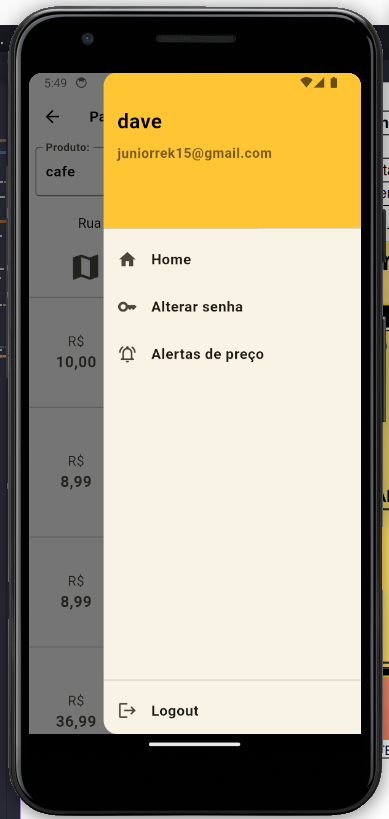
\includegraphics[width=.8\textwidth]{fig/telas/t_mperfil.png}
\footnotesize \centering
\par FONTE: O Autor (2024)
\end{figure}
\end{minipage}
 \\ \hline
\end{tabular}

\subsection*{\textbf{CRITÉRIOS DE ACEITAÇÃO}}

\begin{enumerate}[leftmargin=2cm]
    \item Deve mostrar as informações do usuário logado.
    \item Deve permitir alterar a senha.
    \item Deve permitir configurar alertas de preço.
    \item Deve permitir fazer logout.
\end{enumerate}

\subsection*{\textbf{CRITÉRIOS DE ACEITAÇÃO - DETALHAMENTO}}
\textbf{Critério de contexto} (Válido como premissa para todos os critérios):

\begin{tabularx}{0.9\textwidth}{@{}l X }
 \textbf{Dado que} & Usuário logado. \\ 
 \textbf{E} & Clicou no menu lateral.
\end{tabularx}


\begin{tabularx}{0.9\textwidth}{|l|X|}
\multicolumn{2}{@{}l}{\textbf{1. Deve mostrar as informações do usuário logado.}} \\ \hline
\textbf{Dado que} & Usuário está na tela de perfil. \\ \hline
\textbf{Quando} & Sistema carrega informações do usuário. \\ \hline
\textbf{Então} & Sistema apresenta informações do usuário. \\ \hline
\end{tabularx}

\begin{tabularx}{0.9\textwidth}{|l|X|}
\multicolumn{2}{@{}l}{\textbf{2. Deve permitir alterar a senha.}} \\ \hline
\textbf{Dado que} & Usuário está na tela de perfil. \\ \hline
\textbf{Quando} & Usuário clica em "Alterar senha". \\ \hline
\textbf{Então} & Sistema redireciona para tela de alteração. \\ \hline
\end{tabularx}

\begin{tabularx}{0.9\textwidth}{|l|X|}
\multicolumn{2}{@{}l}{\textbf{3. Deve permitir configurar alertas de preço.}} \\ \hline
\textbf{Dado que} & Usuário está na tela de perfil. \\ \hline
\textbf{Quando} & Usuário clica em "Alertas de preço". \\ \hline
\textbf{Então} & Sistema redireciona para tela de alertas. \\ \hline
\end{tabularx}

\begin{tabularx}{0.9\textwidth}{|l|X|}
\multicolumn{2}{@{}l}{\textbf{4. Deve permitir fazer logout.}} \\ \hline
\textbf{Dado que} & Usuário está na tela de perfil. \\ \hline
\textbf{Quando} & Usuário clica em "Logout". \\ \hline
\textbf{Então} & Sistema redireciona para home e faz logout. \\ \hline
\end{tabularx}



\section{Alterar senha}%%%%%%%%%%%%%%%%%%%%%%%%%%%%%%%%%%%%%

\begin{tabular}{|ll|}
\hline
\multicolumn{2}{|c|}{\textbf{UC\nhist - \currentname}}    \\ \hline
\multicolumn{1}{|l|}{\textbf{Sendo}}     & um usuário \\ \hline
\multicolumn{1}{|l|}{\textbf{Quero}}     & alterar minha senha\\ \hline
\multicolumn{1}{|l|}{\textbf{Para}}      & alterar minha senha atual para uma nova\\ \hline
\multicolumn{1}{|l|}{\textbf{Protótipo}} & 
\begin{minipage}{0.48\textwidth} 
\begin{figure}[H]
\caption{\label{fig:label} TELA ALTERAR SENHA}
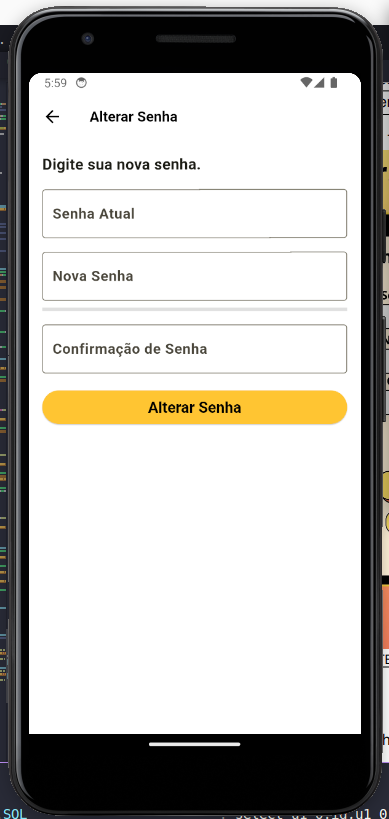
\includegraphics[width=.8\textwidth]{fig/telas/t_altsenha.png}
\footnotesize \centering
\par FONTE: O Autor (2024)
\end{figure}
\end{minipage}
 \\ \hline
\end{tabular}

\subsection*{\textbf{CRITÉRIOS DE ACEITAÇÃO}}

\begin{enumerate}[leftmargin=2cm]
    \item Deve permitir inserir a senha atual e uma nova senha.
    \item Deve permitir alterar a senha caso a senha atual seja inserida corretamente.
\end{enumerate}

\subsection*{\textbf{CRITÉRIOS DE ACEITAÇÃO - DETALHAMENTO}}
\textbf{Critério de contexto} (Válido como premissa para todos os critérios):

\begin{tabularx}{0.9\textwidth}{@{}l X }
\textbf{Dado que} & Usuário logado. \\ 
\textbf{E} & Clicou no menu lateral.\\
\textbf{E} & Clicou em alterar senha.
\end{tabularx}


\begin{tabularx}{0.9\textwidth}{|l|X|}
\multicolumn{2}{@{}l}{\textbf{1. Deve permitir inserir a senha atual e uma nova senha.}} \\ \hline
\textbf{Dado que} & Usuário está na tela de alterar senha. \\ \hline
\textbf{Quando} & Usuário clica nos campos de senha. \\ \hline
\textbf{Então} & Sistema permite inserir dado. \\ \hline
\end{tabularx}

\begin{tabularx}{0.9\textwidth}{|l|X|}
\multicolumn{2}{@{}l}{\textbf{\makecell[l]{2. Deve permitir alterar a senha caso a senha atual seja inserida \\corretamente.}}} \\ \hline
\textbf{Dado que} & Usuário inseriu campos corretamente. (R1) (R2) \\ \hline
\textbf{Quando} & Usuário clicou em "Alterar". \\ \hline
\textbf{Então} & Sistema atualiza senha do usuário. \\ \hline
\end{tabularx}

\subsection*{\textbf{REGRAS DE NEGÓCIO DA HISTÓRIA}}

\begin{itemize}
    \item[] R1 - Senha atual válida.
    \item[] R2 - Novas e confirmação iguais.
\end{itemize}




\section{Logar no sistema}%%%%%%%%%%%%%%%%%%%%%%%%%%%%%%%%%%%%%

\begin{tabular}{|ll|}
\hline
\multicolumn{2}{|c|}{\textbf{UC\nhist - \currentname}}    \\ \hline
\multicolumn{1}{|l|}{\textbf{Sendo}}     & um usuário \\ \hline
\multicolumn{1}{|l|}{\textbf{Quero}}     & logar no sistema\\ \hline
\multicolumn{1}{|l|}{\textbf{Para}}      & poder avaliar e sugerir novos preços para os produtos\\ \hline
\multicolumn{1}{|l|}{\textbf{Protótipo}} & 
\begin{minipage}{0.48\textwidth} 
\begin{figure}[H]
\caption{\label{fig:label} TELA LOGIN}
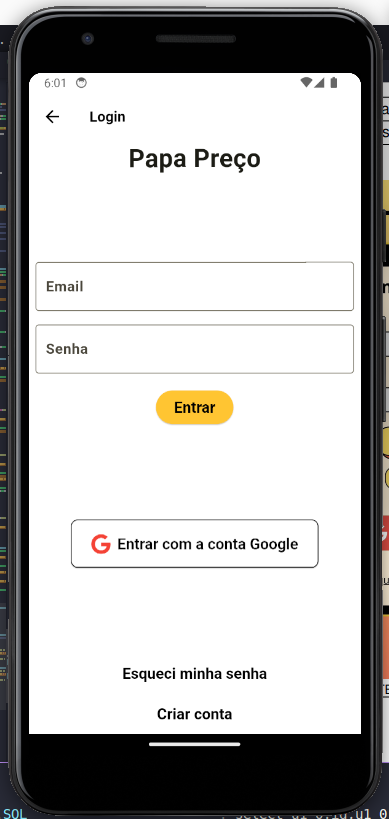
\includegraphics[width=.8\textwidth]{fig/telas/t_login.png}
\footnotesize \centering
\par FONTE: O Autor (2024)
\end{figure}
\end{minipage}
 \\ \hline
\end{tabular}

\subsection*{\textbf{CRITÉRIOS DE ACEITAÇÃO}}

\begin{enumerate}[leftmargin=2cm]
    \item Deve permitir inserir email e senha.
    \item Deve permitir fazer cadastro pela conta Google.
    \item Deve permitir recuperar senha.
    \item Deve permitir acessar formulário de cadastro.
    \item Deve permitir logar no sistema.
\end{enumerate}

\subsection*{\textbf{CRITÉRIOS DE ACEITAÇÃO - DETALHAMENTO}}
\textbf{Critério de contexto} (Válido como premissa para todos os critérios):

\begin{tabularx}{0.9\textwidth}{@{}l X }
 \textbf{Dado que} & Usuário clicou no botão "Login". \\ 
\end{tabularx}


\begin{tabularx}{0.9\textwidth}{|l|X|}
\multicolumn{2}{@{}l}{\textbf{1. Deve permitir inserir email e senha.}} \\ \hline
\textbf{Dado que} & Usuário está na tela de login. \\ \hline
\textbf{Quando} & Usuário clica nos campos. \\ \hline
\textbf{Então} & Sistema permite inserir dado. (R1) (R2) \\ \hline
\end{tabularx}

\begin{tabularx}{0.9\textwidth}{|l|X|}
\multicolumn{2}{@{}l}{\textbf{2. Deve permitir fazer cadastro pela conta Google.}} \\ \hline
\textbf{Dado que} & Usuário está na tela de login. \\ \hline
\textbf{Quando} & Usuário clica no botão Google. \\ \hline
\textbf{Então} & Sistema redireciona para login externo. \\ \hline
\end{tabularx}

\begin{tabularx}{0.9\textwidth}{|l|X|}
\multicolumn{2}{@{}l}{\textbf{3. Deve permitir recuperar senha.}} \\ \hline
\textbf{Dado que} & Usuário está na tela de login. \\ \hline
\textbf{Quando} & Usuário clica em "Esqueci minha senha". \\ \hline
\textbf{Então} & Sistema redireciona para tela de recuperação. \\ \hline
\end{tabularx}

\begin{tabularx}{0.9\textwidth}{|l|X|}
\multicolumn{2}{@{}l}{\textbf{4. Deve permitir acessar formulário de cadastro.}} \\ \hline
\textbf{Dado que} & Usuário está na tela de login. \\ \hline
\textbf{Quando} & Usuário clica em "Criar conta". \\ \hline
\textbf{Então} & Sistema redireciona para tela de cadastro. \\ \hline
\end{tabularx}

\begin{tabularx}{0.9\textwidth}{|l|X|}
\multicolumn{2}{@{}l}{\textbf{5. Deve permitir logar no sistema.}} \\ \hline
\textbf{Dado que} & Usuário inseriu credenciais corretas. (R3) \\ \hline
\textbf{Quando} & Usuário clica em "Entrar". \\ \hline
\textbf{Então} & Sistema autentica usuário e redireciona para tela inicial. \\ \hline
\end{tabularx}

\subsection*{\textbf{REGRAS DE NEGÓCIO DA HISTÓRIA}}

\begin{itemize}
    \item[] R1 - Tamanho maximo do texto 256 caracteres.
    \item[] R2 - Email válido.
    \item[] R3 - Usuário cadastrado no banco de dados.
\end{itemize}

\section{Criar conta}%%%%%%%%%%%%%%%%%%%%%%%%%%%%%%%%%%%%%

\begin{tabular}{|ll|}
\hline
\multicolumn{2}{|c|}{\textbf{UC\nhist - \currentname}}    \\ \hline
\multicolumn{1}{|l|}{\textbf{Sendo}}     & um usuário \\ \hline
\multicolumn{1}{|l|}{\textbf{Quero}}     & cadastrar no sistema\\ \hline
\multicolumn{1}{|l|}{\textbf{Para}}      & criar uma conta para logar no sistema\\ \hline
\multicolumn{1}{|l|}{\textbf{Protótipo}} & 
\begin{minipage}{0.48\textwidth} 
\begin{figure}[H]
\caption{\label{fig:label} TELA CADASTRO}
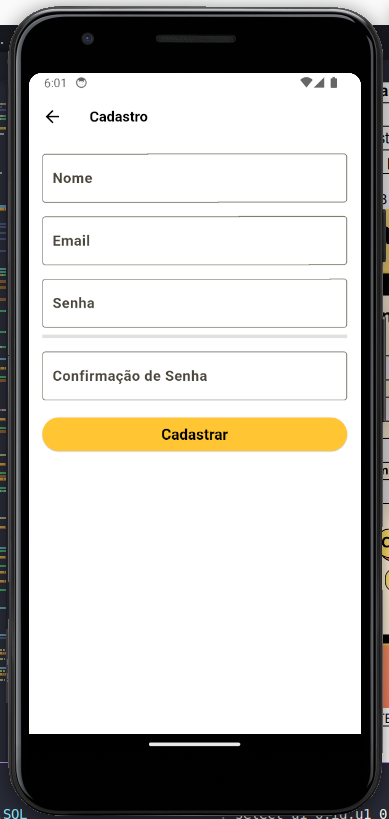
\includegraphics[width=.8\textwidth]{fig/telas/t_cadastro.png}
\footnotesize \centering
\par FONTE: O Autor (2024)
\end{figure}
\end{minipage}
 \\ \hline
\end{tabular}

\subsection*{\textbf{CRITÉRIOS DE ACEITAÇÃO}}

\begin{enumerate}[leftmargin=2cm]
    \item Deve permitir inserir email, nome e senha.
    \item Deve fazer cadastro no sistema.
\end{enumerate}

\subsection*{\textbf{CRITÉRIOS DE ACEITAÇÃO - DETALHAMENTO}}
\textbf{Critério de contexto} (Válido como premissa para todos os critérios):

\begin{tabularx}{0.9\textwidth}{@{}l X }
\textbf{Dado que} & Usuário clicou no botão "Criar conta". \\ 
\end{tabularx}


\begin{tabularx}{0.9\textwidth}{|l|X|}
\multicolumn{2}{@{}l}{\textbf{1. Deve permitir inserir email, nome e senha.}} \\ \hline
\textbf{Dado que} & Usuário está na tela de cadastro. \\ \hline
\textbf{Quando} & Usuário clica nos campos. \\ \hline
\textbf{Então} & Sistema permite inserir dado. \\ \hline
\end{tabularx}

\begin{tabularx}{0.9\textwidth}{|l|X|}
\multicolumn{2}{@{}l}{\textbf{2. Deve fazer cadastro no sistema.}} \\ \hline
\textbf{Dado que} & Usuário preencheu corretamente. (R1) (R2) (R3) (R4) \\ \hline
\textbf{Quando} & Usuário clica em "Cadastrar". \\ \hline
\textbf{Então} & Sistema cadastra novo usuário. \\ \hline
\end{tabularx}

\subsection*{\textbf{REGRAS DE NEGÓCIO DA HISTÓRIA}}

\begin{itemize}
    \item[] R1 - Email válido.
    \item[] R2 - Tamanho máximo do texto 256 caracteres.
    \item[] R3 - Senha e confirmação iguais.
    \item[] R4 - Usuário ainda não cadastrado.
\end{itemize}


\section{Recuperar senha}%%%%%%%%%%%%%%%%%%%%%%%%%%%%%%%%%%%%%

\begin{tabular}{|ll|}
\hline
\multicolumn{2}{|c|}{\textbf{UC\nhist - \currentname}}    \\ \hline
\multicolumn{1}{|l|}{\textbf{Sendo}}     & um usuário \\ \hline
\multicolumn{1}{|l|}{\textbf{Quero}}     & recuperar minha senha\\ \hline
\multicolumn{1}{|l|}{\textbf{Para}}      & acessar o sistema\\ \hline
\multicolumn{1}{|l|}{\textbf{Protótipo}} & 
\begin{minipage}{0.48\textwidth} 
\begin{figure}[H]
\caption{\label{fig:label} TELA RECUPERAR SENHA}
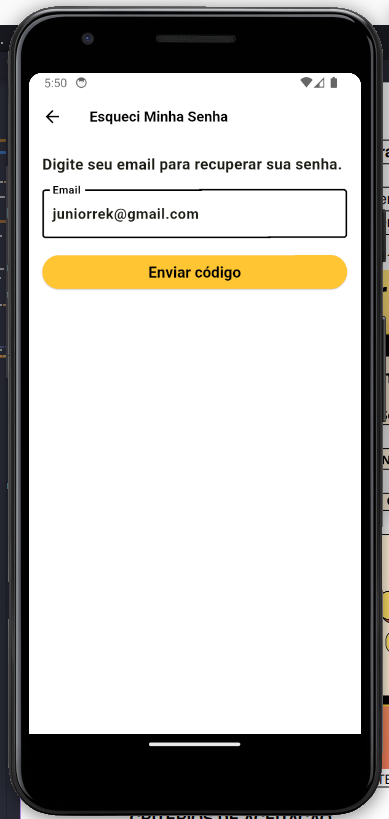
\includegraphics[width=.8\textwidth]{fig/telas/t_esqueci.png}
\footnotesize \centering
\par FONTE: O Autor (2024)
\end{figure}
\end{minipage}
 \\ \hline
\end{tabular}

\subsection*{\textbf{CRITÉRIOS DE ACEITAÇÃO}}

\begin{enumerate}[leftmargin=2cm]
    \item Deve permitir inserir email.
    \item Deve enviar código de verificação para o email cadastrado.
\end{enumerate}

\subsection*{\textbf{CRITÉRIOS DE ACEITAÇÃO - DETALHAMENTO}}
\textbf{Critério de contexto} (Válido como premissa para todos os critérios):

\begin{tabularx}{0.9\textwidth}{@{}l X }
\textbf{Dado que} & Usuário clicou no botão "Esqueci minha senha". \\ 
\end{tabularx}


\begin{tabularx}{0.9\textwidth}{|l|X|}
\multicolumn{2}{@{}l}{\textbf{1. Deve permitir inserir email.}} \\ \hline
\textbf{Dado que} & Usuário está na tela de recuperação. \\ \hline
\textbf{Quando} & Usuário clica no campo "Email". \\ \hline
\textbf{Então} & Sistema permite inserir email. \\ \hline
\end{tabularx}

\begin{tabularx}{0.9\textwidth}{|l|X|}
\multicolumn{2}{@{}l}{\textbf{\makecell[l]{2. Deve enviar código de verificação para o email cadastrado.}}} \\ \hline
\textbf{Dado que} & Usuário preencheu corretamente. (R1) (R2) \\ \hline
\textbf{Quando} & Usuário clica em "Enviar código". \\ \hline
\textbf{Então} & Sistema envia email com código de validação. \\ \hline
\end{tabularx}

\subsection*{\textbf{REGRAS DE NEGÓCIO DA HISTÓRIA}}

\begin{itemize}
    \item[] R1 - Email válido.
    \item[] R2 - Usuário cadastrado.
\end{itemize}


\section{Validar código}%%%%%%%%%%%%%%%%%%%%%%%%%%%%%%%%%%%%%

\begin{tabular}{|ll|}
\hline
\multicolumn{2}{|c|}{\textbf{UC\nhist - \currentname}}    \\ \hline
\multicolumn{1}{|l|}{\textbf{Sendo}}     & um usuário \\ \hline
\multicolumn{1}{|l|}{\textbf{Quero}}     & válidar um código enviado para meu email\\ \hline
\multicolumn{1}{|l|}{\textbf{Para}}      & recuperar minha senha ou verificar meu email\\ \hline
\multicolumn{1}{|l|}{\textbf{Protótipo}} & 
\begin{minipage}{0.48\textwidth} 
\begin{figure}[H]
\caption{\label{fig:label} TELA VALIDAR CÓDIGO}
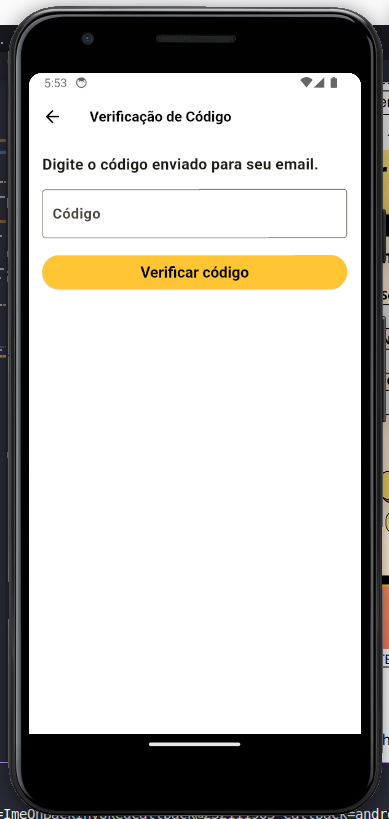
\includegraphics[width=.8\textwidth]{fig/telas/t_validarcodigo.png}
\footnotesize \centering
\par FONTE: O Autor (2024)
\end{figure}
\end{minipage}
 \\ \hline
\end{tabular}

\subsection*{\textbf{CRITÉRIOS DE ACEITAÇÃO}}

\begin{enumerate}[leftmargin=2cm]
    \item Deve permitir inserir código.
    \item Deve validar o código.
\end{enumerate}

\subsection*{\textbf{CRITÉRIOS DE ACEITAÇÃO - DETALHAMENTO}}

\begin{tabularx}{0.9\textwidth}{|l|X|}
\multicolumn{2}{@{}l}{\textbf{1. Deve permitir inserir código.}} \\ \hline
\textbf{Dado que} & Usuário está na tela de validar código. \\ \hline
\textbf{Quando} & Usuário clica no campo "Código". \\ \hline
\textbf{Então} & Sistema permite inserir código. \\ \hline
\end{tabularx}

\begin{tabularx}{0.9\textwidth}{|l|X|}
\multicolumn{2}{@{}l}{\textbf{\makecell[l]{2. Deve validar o código.}}} \\ \hline
\textbf{Dado que} & Usuário preencheu corretamente. (R1) \\ \hline
\textbf{Quando} & Usuário clica em "Verificar código". \\ \hline
\textbf{Então} & Sistema valida o código de validação. \\ \hline
\end{tabularx}

\subsection*{\textbf{REGRAS DE NEGÓCIO DA HISTÓRIA}}

\begin{itemize}
    \item[] R1 - Código válido.
\end{itemize}


\section{Redefinir senha}%%%%%%%%%%%%%%%%%%%%%%%%%%%%%%%%%%%%%

\begin{tabular}{|ll|}
\hline
\multicolumn{2}{|c|}{\textbf{UC\nhist - \currentname}}    \\ \hline
\multicolumn{1}{|l|}{\textbf{Sendo}}     & um usuário \\ \hline
\multicolumn{1}{|l|}{\textbf{Quero}}     & redefinir minha senha\\ \hline
\multicolumn{1}{|l|}{\textbf{Para}}      & alterar minha senha atual\\ \hline
\multicolumn{1}{|l|}{\textbf{Protótipo}} & 
\begin{minipage}{0.48\textwidth} 
\begin{figure}[H]
\caption{\label{fig:label} TELA REDEFINIR SENHA}
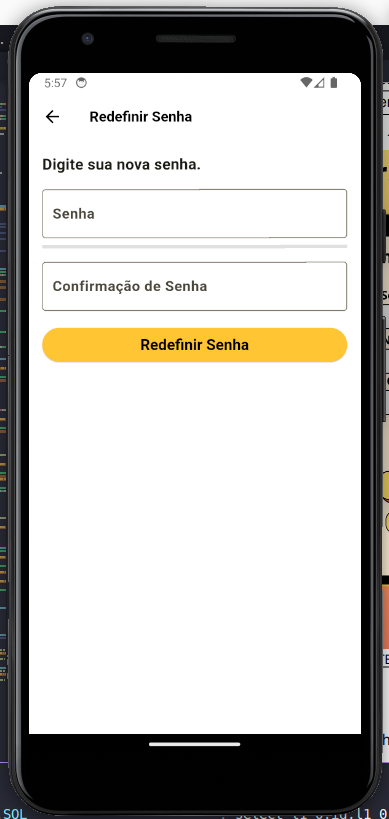
\includegraphics[width=.8\textwidth]{fig/telas/t_redefinirsenha.png}
\footnotesize \centering
\par FONTE: O Autor (2024)
\end{figure}
\end{minipage}
 \\ \hline
\end{tabular}

\subsection*{\textbf{CRITÉRIOS DE ACEITAÇÃO}}

\begin{enumerate}[leftmargin=2cm]
    \item Deve permitir inserir uma nova senha.
    \item Deve permitir alterar a senha.
\end{enumerate}

\subsection*{\textbf{CRITÉRIOS DE ACEITAÇÃO - DETALHAMENTO}}
\textbf{Critério de contexto} (Válido como premissa para todos os critérios):

\begin{tabularx}{0.9\textwidth}{@{}l X }
\textbf{Dado que} & Código válido. \\ 
\end{tabularx}


\begin{tabularx}{0.9\textwidth}{|l|X|}
\multicolumn{2}{@{}l}{\textbf{1. Deve permitir inserir uma nova senha.}} \\ \hline
\textbf{Dado que} & Usuário está na tela de redefinir senha. \\ \hline
\textbf{Quando} & Usuário clica nos campos de senha. \\ \hline
\textbf{Então} & Sistema permite inserir dado. \\ \hline
\end{tabularx}

\begin{tabularx}{0.9\textwidth}{|l|X|}
\multicolumn{2}{@{}l}{\textbf{\makecell[l]{2. Deve permitir alterar a senha.}}} \\ \hline
\textbf{Dado que} & Usuário inseriu campos corretamente. (R1) \\ \hline
\textbf{Quando} & Usuário clicou em "Redefinir". \\ \hline
\textbf{Então} & Sistema atualiza senha do usuário. \\ \hline
\end{tabularx}

\subsection*{\textbf{REGRAS DE NEGÓCIO DA HISTÓRIA}}

\begin{itemize}
    \item[] R1 - Senha e confirmação iguais.
\end{itemize}



\section{Configurar Alertas}%%%%%%%%%%%%%%%%%%%%%%%%%%%%%%%%%%%%%

\begin{tabular}{|ll|}
\hline
\multicolumn{2}{|c|}{\textbf{UC\nhist - \currentname}}    \\ \hline
\multicolumn{1}{|l|}{\textbf{Sendo}}     & um usuário \\ \hline
\multicolumn{1}{|l|}{\textbf{Quero}}     & configurar alertas\\ \hline
\multicolumn{1}{|l|}{\textbf{Para}}      & receber notificações de produtos em um determinado preço\\ \hline
\multicolumn{1}{|l|}{\textbf{Protótipo}} & 
\begin{minipage}{0.48\textwidth} 
\begin{figure}[H]
\caption{\label{fig:label} TELA CONFIGURAR ALERTAS}
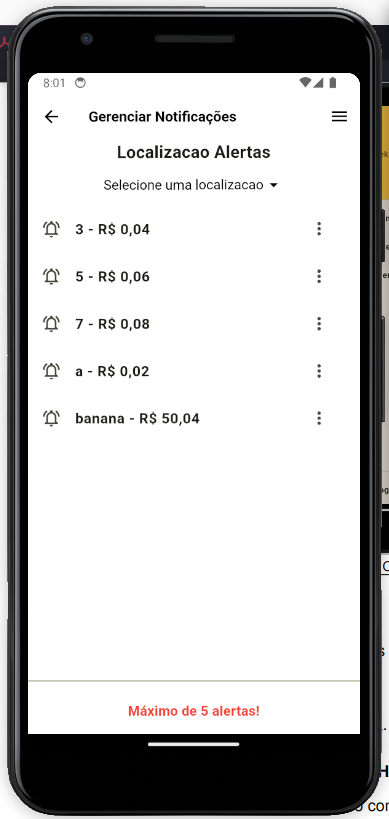
\includegraphics[width=.8\textwidth]{fig/telas/t_gerenciaralertas.png}
\footnotesize \centering
\par FONTE: O Autor (2024)
\end{figure}
\end{minipage}
 \\ \hline
\end{tabular}

\subsection*{\textbf{CRITÉRIOS DE ACEITAÇÃO}}

\begin{enumerate}[leftmargin=2cm]
    \item Deve listar alertas configurados.
    \item Deve permitir inserir/editar/excluir alerta.
    \item Deve permitir definir uma localização.
\end{enumerate}

\subsection*{\textbf{CRITÉRIOS DE ACEITAÇÃO - DETALHAMENTO}}
\textbf{Critério de contexto} (Válido como premissa para todos os critérios):

\begin{tabularx}{0.9\textwidth}{@{}l X }
    \textbf{Dado que} & Usuário logado. \\ 
    \textbf{E} & Acessou tela de alertas através do menu. \\ 
\end{tabularx}


\begin{tabularx}{0.9\textwidth}{|l|X|}
\multicolumn{2}{@{}l}{\textbf{1. Deve listar alertas configurados.}} \\ \hline
\textbf{Dado que} & Usuário está na tela de alertas. \\ \hline
\textbf{Quando} & Entra na tela. \\ \hline
\textbf{Então} & Sistema carregas alertas configurados. \\ \hline
\end{tabularx}

\begin{tabularx}{0.9\textwidth}{|l|X|}
\multicolumn{2}{@{}l}{\textbf{2. Deve permitir inserir/editar/excluir alerta.}} \\ \hline
\textbf{Dado que} & Usuário está na tela de alertas. \\ \hline
\textbf{Quando} & Seleciona algum alerta. \\ \hline
\textbf{Então} & Sistema apresenta formulário de cadastro/edição ou confirmação de exclusão. (R1) \\ \hline
\end{tabularx}

\begin{tabularx}{0.9\textwidth}{|l|X|}
\multicolumn{2}{@{}l}{\textbf{3. Deve permitir definir uma localização.}} \\ \hline
\textbf{Dado que} & Usuário está na tela de alertas. \\ \hline
\textbf{Quando} & Clica em "Selecionar localização". \\ \hline
\textbf{Então} & Sistema redireciona para tela de selecionar localização. \\ \hline
\end{tabularx}

\subsection*{\textbf{REGRAS DE NEGÓCIO DA HISTÓRIA}}

\begin{itemize}
    \item[] R1 - Máximo de 5 alertas por usuário.
\end{itemize}
